\documentclass[11pt]{article}

\usepackage[margin=1in]{geometry}
\usepackage{amsmath}
\usepackage{graphicx}
\usepackage{caption}
\usepackage{booktabs}
\usepackage{xcolor}
\usepackage{listings}
\usepackage{needspace}
\usepackage{placeins}
\usepackage[hidelinks]{hyperref}

\captionsetup{hypcap=false}

\raggedbottom
\clubpenalty=500
\widowpenalty=500
\displaywidowpenalty=500

\let\oldsection\section
\renewcommand{\section}[1]{\Needspace{3\baselineskip}\oldsection{#1}}

\let\oldsubsection\subsection
\renewcommand{\subsection}[1]{\Needspace{2\baselineskip}\oldsubsection{#1}}

\lstdefinestyle{cppstyle}{
    language=C++,
    basicstyle=\ttfamily\small,
    keywordstyle=\color{blue!60!black},
    commentstyle=\color{green!40!black},
    stringstyle=\color{red!60!black},
    frame=single,
    breaklines=true,
    showstringspaces=false,
    aboveskip=0.45em,
    belowskip=0.45em
}

\setlength{\parskip}{5pt plus 1pt}
\setlength{\parindent}{0pt}

\title{Documentation and Results for the 2D Ising Model}
\author{Jacob Emmanuel Sadorra}
\date{June 2026}

\begin{document}

\maketitle

\section{Documentation}

\subsection{Background of the 2D Ising Model}

The two-dimensional Ising model is a standard model for studying magnetic ordering and phase transitions in statistical mechanics \cite{chandler1987,pathria2011}. The system is an $N \times N$ square lattice of spins, where each spin has value $s_i=\pm 1$. For the ferromagnetic case, the energy is

\medskip

\begin{equation}
E=-J\sum_{\langle i,j\rangle}s_i s_j,
\end{equation}

\medskip
where the sum is over nearest-neighbor pairs. In this project $J=1$, so aligned neighboring spins lower the energy and anti-aligned neighboring spins raise it.

Temperature is written using the dimensionless parameter

\medskip

\begin{equation}
\alpha=\frac{k_B T}{J}.
\end{equation}

\medskip
At small $\alpha$, the spins tend to align and the system is magnetized. At large $\alpha$, thermal fluctuations dominate and the lattice becomes disordered. Onsager's exact solution for the infinite two-dimensional square lattice gives the critical value \cite{onsager1944}

\medskip

\begin{equation}
\alpha_c=\frac{2}{\ln(1+\sqrt{2})}\approx 2.269,
\end{equation}

\medskip
but finite lattices such as $N=20$ and $N=40$ show a rounded transition rather than a perfectly sharp singularity.

\subsection{Program Structure}

The simulation in \texttt{Ising\_Model.cpp} is organized around an \texttt{ising} class. This class keeps the lattice size, the spin array, the random number generator, and the functions needed for initialization, energy calculation, magnetization calculation, and Metropolis updates. The main data members are shown below.

\Needspace{5\baselineskip}
\begin{lstlisting}[style=cppstyle]
class ising {
public:
    int N;
    int spins;
    std::vector<std::vector<int>> spin;
    std::uniform_int_distribution<int> random_site;
    std::bernoulli_distribution coin;
    std::uniform_real_distribution<double> unif_dis;
    std::random_device rd;
    std::mt19937 rng;
};
\end{lstlisting}

The lattice is stored as a two-dimensional \texttt{vector}. The random number generator is \texttt{std::mt19937}, and it is seeded with \texttt{std::random\_device}. This avoids repeating the same random trajectory every time the program is run. Random numbers are used when the initial spin configuration is made, when trial spin-flip sites are selected, and when the Metropolis acceptance test is applied.

The constructor prepares the lattice and the random distributions used throughout the simulation:

\Needspace{5\baselineskip}
\begin{lstlisting}[style=cppstyle]
ising(int lattice_size)
    : N(lattice_size),
    spins(lattice_size * lattice_size),
    spin(lattice_size, std::vector<int>(lattice_size)),
    random_site(0, lattice_size - 1),
    coin(0.5),
    unif_dis(0.0, 1.0),
    rng(rd())
{}
\end{lstlisting}

\subsection{Lattice Initialization and Boundary Conditions}

At the start of each temperature calculation, the lattice is initialized randomly. Each spin is assigned $+1$ or $-1$ with equal probability:

\Needspace{4\baselineskip}
\begin{lstlisting}[style=cppstyle]
if (coin(rng) == 1) {
    spin[i][j] = 1;
}
else {
    spin[i][j] = -1;
}
\end{lstlisting}

Periodic boundary conditions are implemented directly when the nearest neighbors are accessed. For example, the four neighbors of site $(i,j)$ are selected as:

\Needspace{4\baselineskip}
\begin{lstlisting}[style=cppstyle]
int up = spin[i][(j+1)%N];
int down = spin[i][(j-1+N)%N];
int right = spin[(i+1)%N][j];
int left = spin[(i-1+N)%N][j];
\end{lstlisting}

The modulo operation makes the lattice wrap around at the edges. This reduces artificial boundary effects, since a spin on one edge still has neighbors on the opposite edge.

\subsection{Metropolis Algorithm}

For each trial update, one lattice site is chosen randomly and its spin is temporarily flipped. The energy change is calculated using only the four nearest neighbors, which is more efficient than recalculating the total lattice energy after every trial move:

\medskip

\begin{equation}
\Delta E=-2s_{i,j}^{\mathrm{new}}
\left(s_{\mathrm{up}}+s_{\mathrm{down}}+s_{\mathrm{left}}+s_{\mathrm{right}}\right).
\end{equation}

\medskip
If $\Delta E \leq 0$, the move is accepted. If $\Delta E>0$, the move is accepted with probability

\medskip

\begin{equation}
P_{\mathrm{accept}}=e^{-\Delta E/\alpha}.
\end{equation}

\medskip
If the move is rejected, the spin is flipped back to its previous value. This local accept-or-reject step is the main update rule used in the code:

\Needspace{7\baselineskip}
\begin{lstlisting}[style=cppstyle]
i = random_site(rng);
j = random_site(rng);
spin[i][j] *= -1;

int up = spin[i][(j+1)%N];
int down = spin[i][(j-1+N)%N];
int right = spin[(i+1)%N][j];
int left = spin[(i-1+N)%N][j];

double dE = -2 * (spin[i][j] * (up + down + right + left));

if (dE <= 0) {
    return true;
}
else {
    double probability = std::exp(-dE / T);
    if (unif_dis(rng) < probability) {
        return true;
    }
    else {
        spin[i][j] *= -1;
        return false;
    }
}
\end{lstlisting}

One Monte Carlo sweep is defined as $N^2$ attempted spin flips, so each spin has approximately one chance to be updated per sweep. For each temperature, the code first performs $100{,}000$ equilibration sweeps and then performs $300{,}000$ sampling sweeps. Measurements are collected only after equilibration.

\subsection{Measured Quantities}

The total magnetization is

\medskip

\begin{equation}
M=\sum_i s_i.
\end{equation}

\medskip
The output uses $|M|$ because a finite lattice can switch between positive and negative magnetized states even below the transition temperature. Taking the absolute value prevents these sign changes from canceling the ordered state in the average.

The total energy is calculated as

\medskip

\begin{equation}
E=-\frac{1}{2}\sum_i s_i
\left(s_{\mathrm{up}}+s_{\mathrm{down}}+s_{\mathrm{left}}+s_{\mathrm{right}}\right).
\end{equation}

\medskip
The factor $1/2$ is included because each nearest-neighbor pair is counted twice in the site-by-site sum.

After sampling, the stored averages of $E$, $E^2$, $|M|$, and $M^2$ are used to calculate the heat capacity and susceptibility:

\medskip

\begin{equation}
\frac{C_V}{N^2}
=
\frac{\langle E^2\rangle-\langle E\rangle^2}
{\alpha^2N^2}
\end{equation}

\medskip
and

\medskip

\begin{equation}
\frac{\chi}{N^2}
=
\frac{\langle M^2\rangle-\langle |M|\rangle^2}
{\alpha N^2}.
\end{equation}

\medskip
The program also records the Metropolis acceptance ratio:

\medskip

\begin{equation}
\frac{\text{accepted moves}}{\text{accepted moves}+\text{rejected moves}}.
\end{equation}

The following part of the code shows how measurements are taken once per sweep after the equilibration period:

\Needspace{5\baselineskip}
\begin{lstlisting}[style=cppstyle]
if ((r+1) % sweep == 0) {
    if (r >= equilibriation_sweep * sweep) {
        double Ef = model.total_energy_i(0, 0);
        double Mf = model.calculate_total_magnetization();
        E = E + Ef;
        E_2 = E_2 + Ef * Ef;
        M = M + std::abs(Mf);
        M_2 = M_2 + Mf * Mf;
        samples++;
    }
}
\end{lstlisting}

\subsection{Simulation Range and Output}

The function \texttt{simulation(N)} runs the calculation from $\alpha=1.00$ to $\alpha=4.00$ with step size $\Delta\alpha=0.01$. The temperature loop is controlled by an integer index, which avoids repeatedly adding a floating-point value and helps keep the temperature values consistent:

\Needspace{4\baselineskip}
\begin{lstlisting}[style=cppstyle]
int temperature_points =
    static_cast<int>(std::round((Tmax - Tmin) / step_add)) + 1;

for (int temp_index = 0; temp_index < temperature_points; temp_index++) {
    double alpha = Tmin + temp_index * step_add;
    ...
}
\end{lstlisting}

The \texttt{main()} function runs the same simulation for both lattice sizes:

\Needspace{4\baselineskip}
\begin{lstlisting}[style=cppstyle]
int main() {
    simulation(20);
    simulation(40);
    return 0;
}
\end{lstlisting}

This produces two output files:

\begin{center}
\begin{tabular}{ll}
\toprule
Lattice size & Output file \\
\midrule
$N=20$ & \texttt{ising\_data\_N20.csv} \\
$N=40$ & \texttt{ising\_data\_N40.csv} \\
\bottomrule
\end{tabular}
\end{center}

Each CSV file stores the temperature parameter, average energy, energy per spin, average absolute magnetization, magnetization per spin, specific heat per spin, susceptibility per spin, and acceptance ratio. The plotting script \texttt{plot\_ising\_results.py} reads these CSV files and generates the graphs used in the results section.

\section{Results}

\subsection{Expected Critical Temperature}

For the infinite two-dimensional square-lattice Ising model with zero external field, the exact critical temperature from Onsager's solution is \cite{onsager1944}

\medskip

\begin{equation}
\alpha_c = \frac{2}{\ln(1+\sqrt{2})} \approx 2.269.
\end{equation}

\medskip
The finite-size Monte Carlo simulations should show transition behavior near this value, although the peaks are expected to be broadened and possibly shifted because $N=20$ and $N=40$ are finite systems.

For comparison with the magnetization result, the exact infinite-lattice spontaneous magnetization is also plotted. This expression was announced by Onsager and later derived by Yang \cite{onsager1944,yang1952}:

\medskip

\begin{equation}
m_{\mathrm{exact}}(\alpha)=
\begin{cases}
\left[1-\sinh^{-4}\left(\frac{2}{\alpha}\right)\right]^{1/8},
& \alpha<\alpha_c, \\
0,
& \alpha\geq\alpha_c .
\end{cases}
\end{equation}

\medskip

\subsection{Summary of Observables}

Figure~\ref{fig:summary} shows the four main observables used to study the two-dimensional Ising model: average energy, magnetization, specific heat, and magnetic susceptibility. Together, these quantities show how the lattice changes from an ordered low-temperature state to a more disordered high-temperature state. The energy and magnetization describe the average state of the system, while the specific heat and susceptibility highlight the fluctuation behavior near the transition region.

\begin{figure}[!htbp]
    \centering
    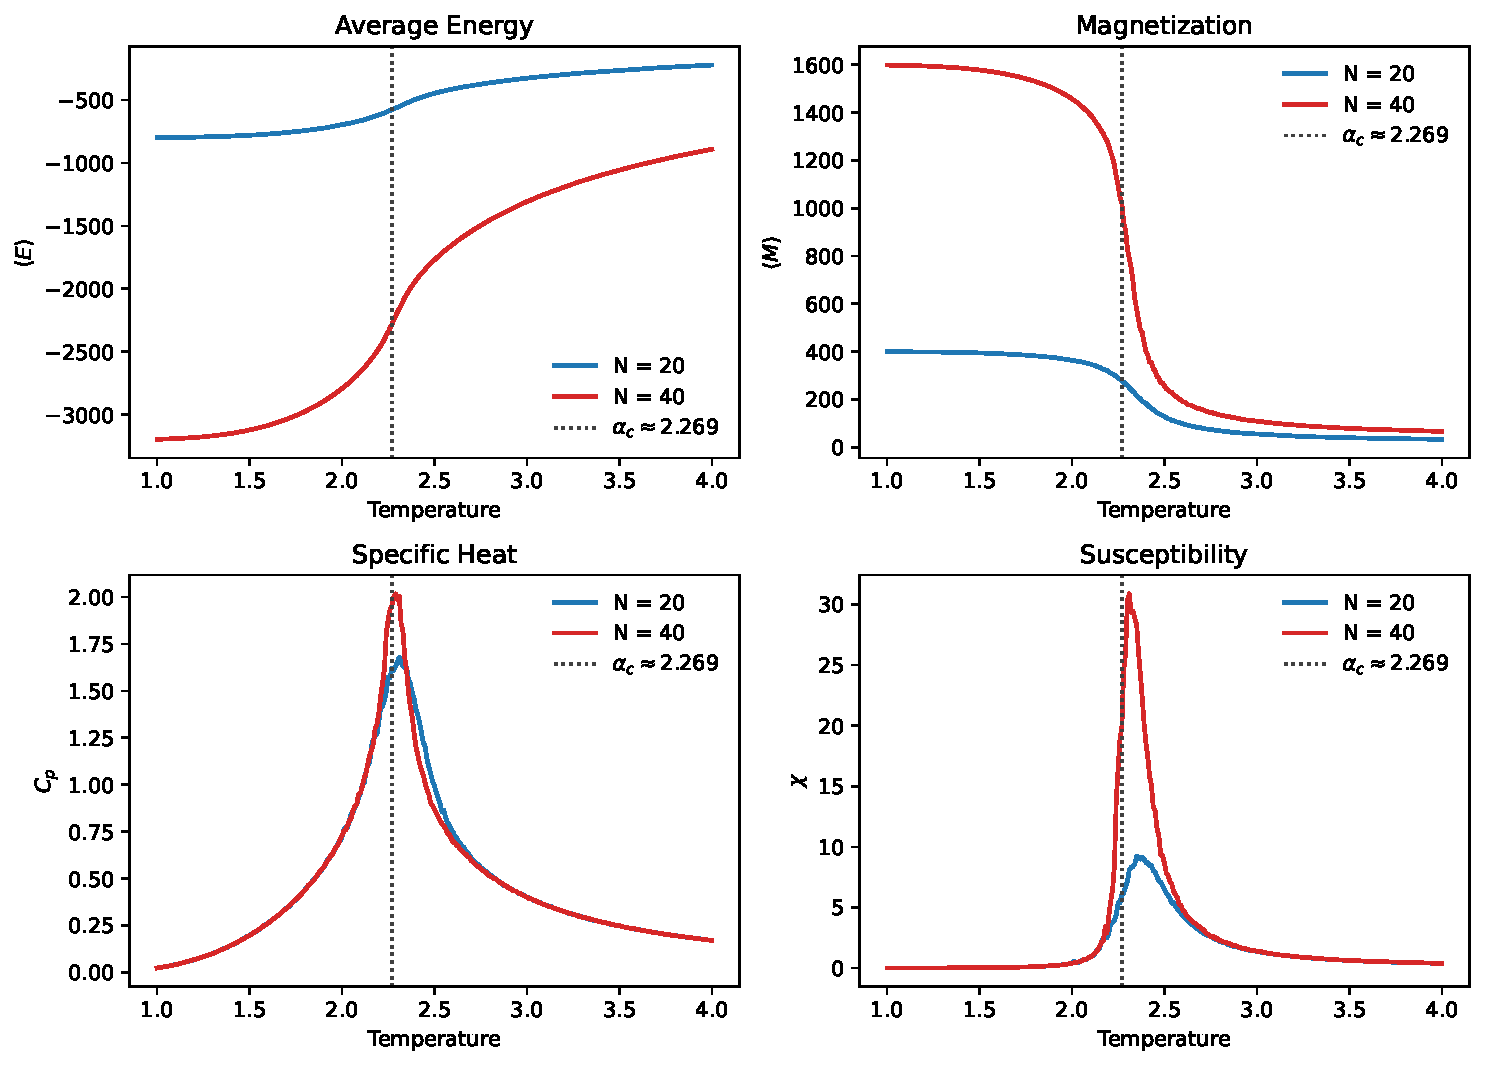
\includegraphics[width=\textwidth]{figures/ising_observables_summary.pdf}
    \caption{Monte Carlo simulation results for $N=20$ and $N=40$. The vertical dotted line marks the exact critical value $\alpha_c \approx 2.269$. Approximate runtime: 2 h.}
    \label{fig:summary}
\end{figure}
\FloatBarrier

\subsection{Energy}

\noindent
\begin{minipage}[c]{0.42\textwidth}
Figure~\ref{fig:energy} shows that the average energy starts very negative at low $\alpha$, where most neighboring spins are aligned. As the temperature parameter increases, misaligned neighbors become more common and the energy moves upward toward zero. The curve is steepest near the transition region rather than changing uniformly across the full temperature range. This rapid but still rounded change is expected for a finite Ising lattice, where the sharp thermodynamic-limit transition is softened by finite size \cite{chandler1987,pathria2011}.
\end{minipage}
\hfill
\begin{minipage}[c]{0.54\textwidth}
    \centering
    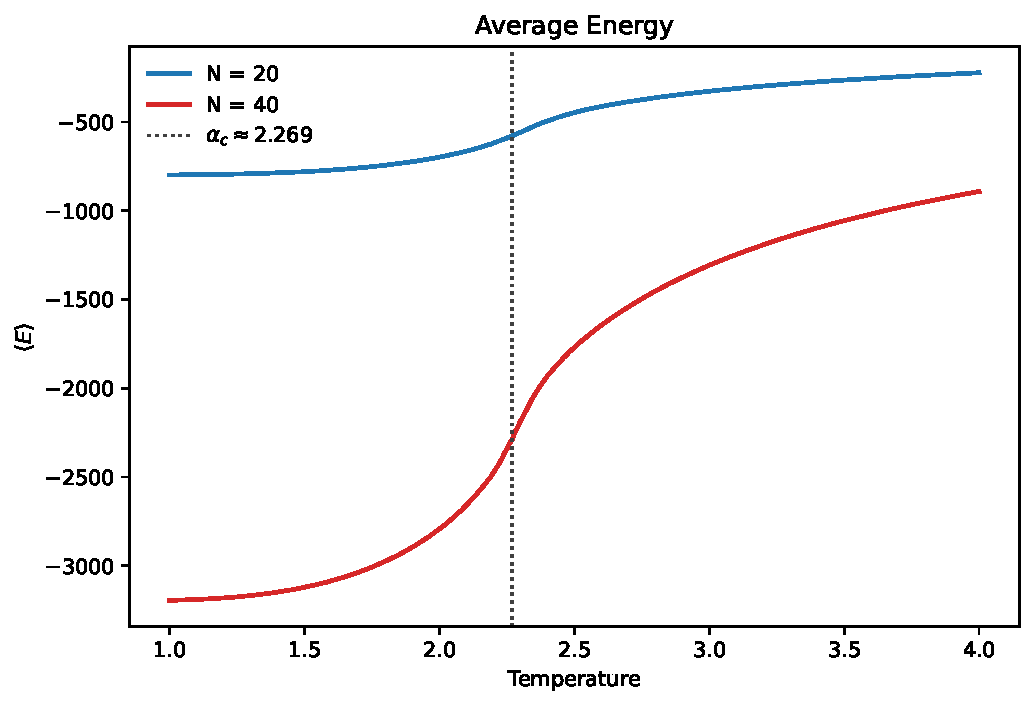
\includegraphics[width=\linewidth]{figures/ising_energy.pdf}
    \captionof{figure}{Average energy as a function of temperature.}
    \label{fig:energy}
\end{minipage}

\medskip

\subsection{Magnetization}

\noindent
\begin{minipage}[c]{0.42\textwidth}
Figure~\ref{fig:magnetization} shows the magnetization normalized by $N^2$. This makes the two lattice sizes easier to compare and allows the Onsager-Yang result to be shown on the same scale. At low $\alpha$, the normalized magnetization is close to 1, so the lattice is strongly ordered. Near $\alpha_c$, it drops quickly, showing the loss of long-range spin alignment. The Monte Carlo curves follow the exact result well at low temperature, then round off near the transition because finite lattices cannot show a true singularity.
\end{minipage}
\hfill
\begin{minipage}[c]{0.54\textwidth}
    \centering
    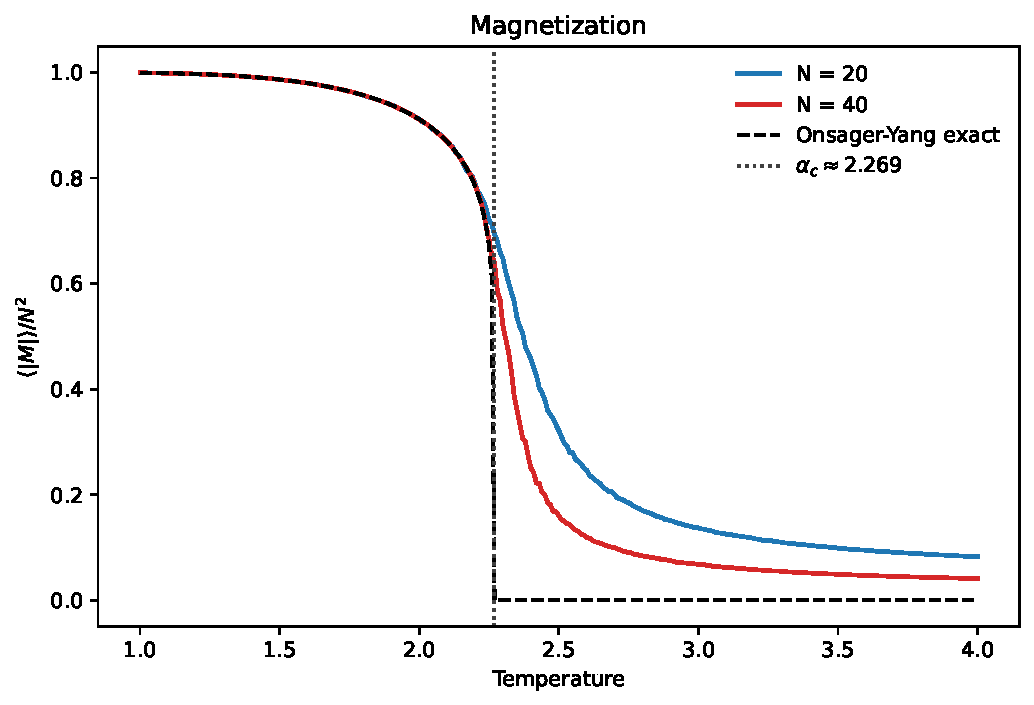
\includegraphics[width=\linewidth]{figures/ising_magnetization.pdf}
    \captionof{figure}{Average magnetization normalized by $N^2$, with the exact Onsager-Yang magnetization shown as a dashed curve.}
    \label{fig:magnetization}
\end{minipage}

\medskip

\subsection{Specific Heat}

\noindent
\begin{minipage}[c]{0.42\textwidth}
Figure~\ref{fig:specific_heat} shows a clear peak in the specific heat near the critical region. The peak occurs near $\alpha \approx 2.31$ for $N=20$ and near $\alpha \approx 2.29$ for $N=40$, close to $\alpha_c \approx 2.269$. This is a useful transition indicator because heat capacity measures energy fluctuations \cite{chandler1987,pathria2011}. The $N=40$ peak is sharper, which suggests that increasing the lattice size is moving the result closer to thermodynamic-limit behavior.
\end{minipage}
\hfill
\begin{minipage}[c]{0.54\textwidth}
    \centering
    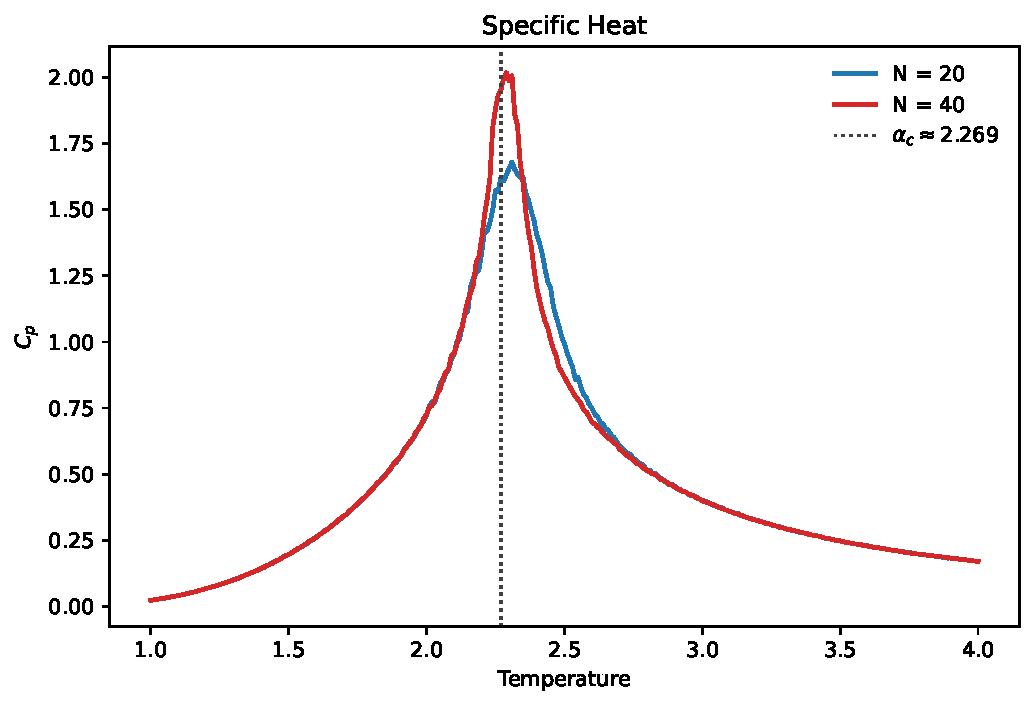
\includegraphics[width=\linewidth]{figures/ising_specific_heat.pdf}
    \captionof{figure}{Specific heat as a function of temperature.}
    \label{fig:specific_heat}
\end{minipage}

\medskip

\subsection{Magnetic Susceptibility}

\noindent
\begin{minipage}[c]{0.42\textwidth}
Figure~\ref{fig:susceptibility} shows that the susceptibility also rises sharply near the transition. The peak is near $\alpha \approx 2.35$ for $N=20$ and near $\alpha \approx 2.31$ for $N=40$. Since susceptibility comes from magnetization fluctuations, this peak means that the spin ordering is most unstable in the critical region \cite{pathria2011,landau2009}. The taller $N=40$ peak is another sign that the transition becomes more pronounced for larger systems.
\end{minipage}
\hfill
\begin{minipage}[c]{0.54\textwidth}
    \centering
    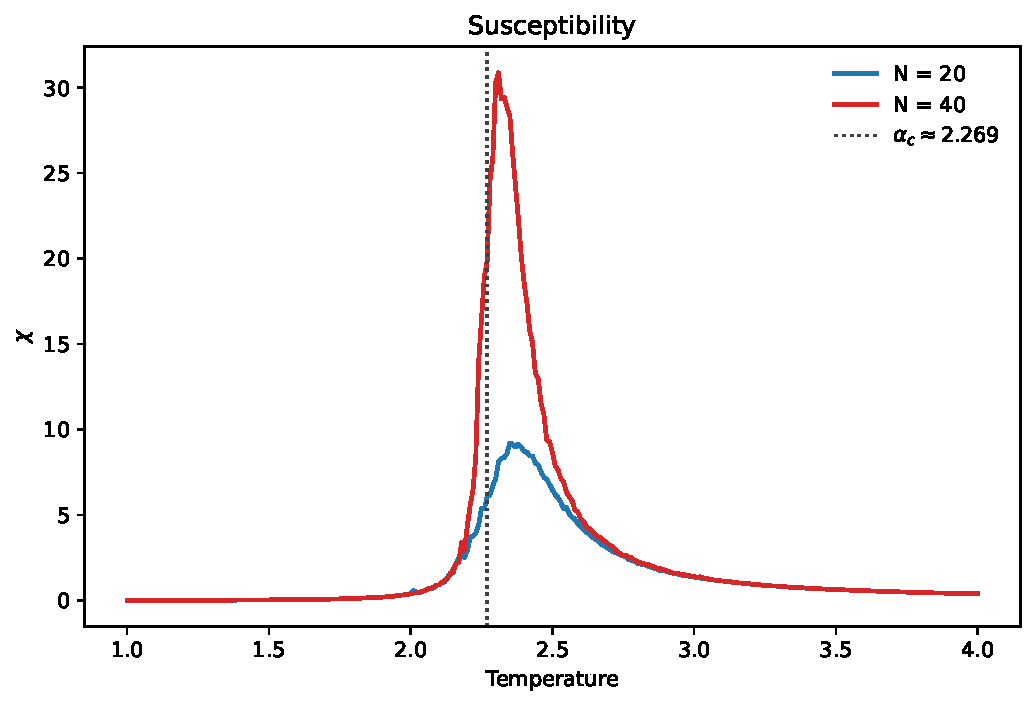
\includegraphics[width=\linewidth]{figures/ising_susceptibility.pdf}
    \captionof{figure}{Magnetic susceptibility as a function of temperature.}
    \label{fig:susceptibility}
\end{minipage}

\medskip

\subsection{Acceptance Ratio}

\noindent
\begin{minipage}[c]{0.42\textwidth}
Figure~\ref{fig:acceptance} shows the Metropolis acceptance ratio. At low temperature, many proposed spin flips would increase the energy, so they are rejected. At higher temperature, those energetically unfavorable flips are accepted more often. The increasing acceptance ratio is therefore consistent with the lattice becoming more disordered as thermal fluctuations become stronger.
\end{minipage}
\hfill
\begin{minipage}[c]{0.54\textwidth}
    \centering
    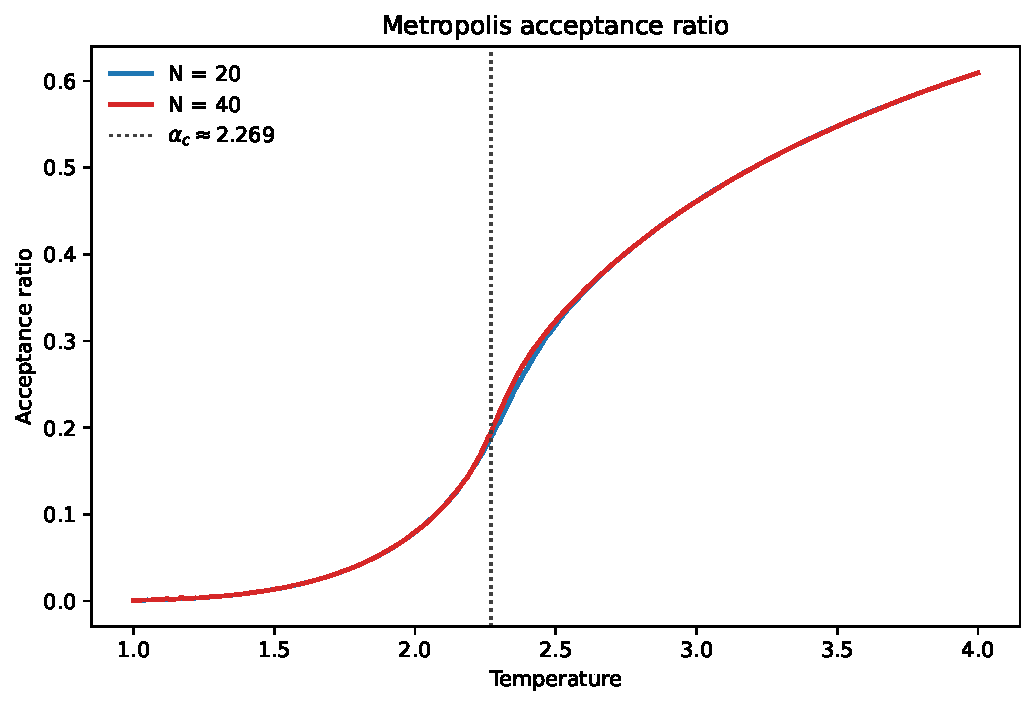
\includegraphics[width=\linewidth]{figures/ising_acceptance_ratio.pdf}
    \captionof{figure}{Metropolis acceptance ratio as a function of temperature.}
    \label{fig:acceptance}
\end{minipage}

\medskip

\subsection{Spin Configuration Behavior}

The spin configurations should change from ordered to disordered as $\alpha$ increases. At low $\alpha$, most spins are part of one large aligned region, so the lattice has a strong net magnetization. Near $\alpha_c$, large clusters of up and down spins can both appear, and the configuration changes more strongly from one sampled state to another. At high $\alpha$, the lattice is much more mixed, with neighboring spins less strongly correlated. This visual picture matches the drop in magnetization and the peaks in the fluctuation-based quantities near the transition.

\subsection{Finite-Size Comparison}

The $N=20$ and $N=40$ simulations show the same overall trend, but the larger lattice has sharper features near the transition. This is most visible in Figures~\ref{fig:magnetization}, \ref{fig:specific_heat}, and \ref{fig:susceptibility}. A finite lattice cannot produce the true mathematical singularity of the infinite system. Instead, the transition appears as a rounded change. As $N$ increases, the rounded behavior is expected to become sharper and move closer to the thermodynamic-limit result.

\section{Additional Analysis on the Monte Carlo Method}

\subsection{Question 1: Noisy Specific Heat and Susceptibility}

In the example shown in the project guideline, the average energy and magnetization look reasonable, but the specific heat and susceptibility fluctuate strongly. This can happen because $C_V$ and $\chi$ are calculated from fluctuations, not just from direct averages \cite{chandler1987,pathria2011,landau2009}:

\medskip

\begin{equation}
\frac{C_V}{N^2}
=
\frac{\langle E^2\rangle-\langle E\rangle^2}{\alpha^2N^2},
\end{equation}

\medskip
\begin{equation}
\frac{\chi}{N^2}
=
\frac{\langle M^2\rangle-\langle |M|\rangle^2}{\alpha N^2}.
\end{equation}

\medskip
Since these formulas subtract two large averaged quantities, small statistical errors can become much more visible in the final curves. The main statistical problem is autocorrelation: nearby Monte Carlo configurations are not fully independent, especially near the critical temperature \cite{landau2009}. If correlated configurations are treated as independent samples, the averages may look stable while the fluctuation-based quantities remain noisy. Increasing the number of Monte Carlo steps can reduce the noise, but it is costly because many added samples may still be correlated.

The present code reduces this issue in two ways. First, it discards $100{,}000$ equilibration sweeps before taking measurements, so the random initial configuration has less influence on the averages. Second, it measures only once per sweep rather than after every attempted spin flip:

\medskip

\begin{equation}
\text{one sample} \quad \text{after} \quad N^2 \text{ attempted spin flips}.
\end{equation}

\medskip
This does not completely remove autocorrelation, but it gives the lattice more time to change between measurements. The code also uses $300{,}000$ sampling sweeps, which improves the statistics compared with a much shorter run. Therefore, the code avoids the worst version of the problem by separating equilibration from measurement and by not recording every attempted spin flip as an independent data point.

The equilibration step appears directly in the sampling condition:

\Needspace{5\baselineskip}
\begin{lstlisting}[style=cppstyle]
if ((r+1) % sweep == 0) {
    if (r >= equilibriation_sweep * sweep) {
        double Ef = model.total_energy_i(0, 0);
        double Mf = model.calculate_total_magnetization();
        E = E + Ef;
        M = M + std::abs(Mf);
        samples++;
    }
}
\end{lstlisting}

This means that the first $100{,}000$ sweeps are used only to relax the system. Measurements of $E$ and $M$ begin only after the condition \texttt{r >= equilibriation\_sweep * sweep} is satisfied.

\subsection{Question 2: Monte Carlo in Chemistry}

An example related to chemistry is the work by Patel et al. on a supported organovanadium(III) hydrogenation catalyst \cite{patel2021}. The central problem is active-site heterogeneity: a supported catalyst can contain many slightly different local environments, so one idealized active site may not represent the full catalytic behavior.

In this paper, Monte Carlo was used as kinetic Monte Carlo rather than as equilibrium Metropolis sampling. The workflow was to first use DFT to calculate free-energy barriers for possible elementary steps in styrene hydrogenation. These barriers were then converted into rate constants using transition state theory. In simplified form, each possible event $i$ has a rate constant

\medskip

\begin{equation}
k_i \propto e^{-\Delta G_i^\ddagger / RT}.
\end{equation}

\medskip
During the kinetic Monte Carlo simulation, a reaction event is chosen with probability

\medskip

\begin{equation}
P_i=\frac{k_i}{\sum_j k_j}.
\end{equation}

\medskip
Therefore, faster elementary steps are more likely to occur, but slower events can still happen. This allows the simulation to follow the time evolution of many catalyst sites and many possible reaction events.

Monte Carlo-style sampling is useful for this kind of problem because it can sample many possible microscopic environments and estimate an ensemble-averaged behavior instead of relying on only one structure. In a heterogeneous catalyst, different sites can have different reaction barriers or different probabilities of being occupied. Rate-weighted sampling helps determine whether the observed catalytic behavior is controlled by one dominant site type or by a distribution of active sites.

The main limitation is that the result still depends on the underlying energetic model and on how well the sampled sites represent the real catalyst. If important active sites are missing from the model, or if the calculated barriers are inaccurate, the averaged prediction can still be biased. Monte Carlo sampling improves the treatment of heterogeneity, but it cannot fix an incomplete physical model by itself.

\begin{thebibliography}{9}

\bibitem{chandler1987}
D. Chandler,
\textit{Introduction to Modern Statistical Mechanics},
Oxford University Press, New York, 1987.

\bibitem{pathria2011}
R. K. Pathria and P. D. Beale,
\textit{Statistical Mechanics}, 3rd ed.,
Elsevier/Academic Press, Oxford, 2011.

\bibitem{landau2009}
D. P. Landau and K. Binder,
\textit{A Guide to Monte Carlo Simulations in Statistical Physics}, 3rd ed.,
Cambridge University Press, Cambridge, 2009.

\bibitem{onsager1944}
L. Onsager,
``Crystal Statistics. I. A Two-Dimensional Model with an Order-Disorder Transition,''
\textit{Physical Review}, vol. 65, pp. 117--149, 1944.
doi: \href{https://doi.org/10.1103/PhysRev.65.117}{10.1103/PhysRev.65.117}.

\bibitem{yang1952}
C. N. Yang,
``The Spontaneous Magnetization of a Two-Dimensional Ising Model,''
\textit{Physical Review}, vol. 85, pp. 808--816, 1952.
doi: \href{https://doi.org/10.1103/PhysRev.85.808}{10.1103/PhysRev.85.808}.

\bibitem{patel2021}
P. Patel, R. H. Wells, D. M. Kaphan, M. Delferro, R. T. Skodje, and C. Liu,
``Computational Investigation of the Role of Active Site Heterogeneity for a Supported Organovanadium(III) Hydrogenation Catalyst,''
\textit{ACS Catalysis}, vol. 11, pp. 7257--7269, 2021.
doi: \href{https://doi.org/10.1021/acscatal.1c00688}{10.1021/acscatal.1c00688}.

\end{thebibliography}

\end{document}
